\documentclass[article,12pt]{article}

\usepackage[utf8]{inputenc}
\usepackage{amssymb, amsfonts,amsthm}
\usepackage[fleqn]{amsmath} % Math packages
\numberwithin{equation}{section}
\usepackage{listings}
\usepackage[top=1in, bottom=1in, left=1in, right=1in]{geometry}
%\usepackage[T1]{fontenc} % Use 8-bit encoding that has 256 glyphs
%\usepackage{fourier} % Use the Adobe Utopia font for the document - comment this line to return to the LaTeX default
\usepackage[english]{babel} % English language/hyphenation
\usepackage{enumerate}
\usepackage[usenames,dvipsnames]{color} % Required for custom colors
\usepackage{listings} % Required for insertion of code
\usepackage{courier} % Required for the courier font
\usepackage{tikz} 
\usepackage{sectsty}
\usepackage{multicol} % Required for multiple columns
%\usepackage{tabu} % Option for Table Construction
\usepackage{epigraph} 
\setlength{\epigraphwidth}{\textwidth}
\usepackage{hologo}
\usepackage[font=small,labelfont=bf]{caption} % Specifying Captions
\usepackage{multirow} % TAbles
\usepackage{changepage} % Change margins



\usepackage{blindtext}
\usepackage{setspace} % Spacing
\usepackage{csquotes}% Recommended
\usepackage{psvectorian} % Cool ornaments

\usepackage{hyperref} % hyper links
\hypersetup{
	colorlinks=true,
	linkcolor=blue,
	filecolor=magenta,      
	urlcolor=cyan,
	pdftitle={Rob's GIS 5571 Final Report},
	pdfpagemode=FullScreen,
	citecolor= black
}

\urlstyle{same}


\renewcommand{\baselinestretch}{1.5} % Spacing

\usepackage[style = numeric, sorting = none, backend=biber]{biblatex}
\addbibresource{references.bib}

\usepackage{graphicx}
\graphicspath{{figs/}} %Setting the graphicspath


\begin{document}

\begin{center}
\textbf{Final Report}

Title: Measuring the Distribution of Air Quality Hazards Across Minneapolis\\
Notice: Dr. Bryan Runck\\
Author: Rob Hendrickson\\
Date: 12/21/2022\\~\\

Project Repository: \url{https://github.com/RwHendrickson/GIS5571/blob/main/Final_Project}\\
Time Spent: 70+ hours

\end{center}
\vspace{1in}
The EPA defines environmental justice as: 
\begin{displayquote}
	“...the fair treatment and meaningful involvement of all people regardless of race, color, national origin, or income with respect to the development, implementation and enforcement of environmental laws, regulations and policies. Fair treatment means no group of people should bear a disproportionate share of the negative environmental consequences resulting from industrial, governmental and commercial operations or policies.” \cite{epaEJ} 
\end{displayquote}
\vspace{0.5in}
\section*{Abstract}
It is understood that some parts of Minneapolis experience a greater burden of environmental hazard than others. Anecdotally and visually, this can be correlated to restrictive housing practices of the early to mid 20th century. This project aims to quantify the cumulative environmental harms across Minneapolis at a fine spatial resolution with the intention of spatially correlating this with modern demographics and restrictive housing practices.


\section{Problem Statement}

From the colonization of the sacred Bdote Region of the Dakota people to the first racially restrictive \href{https://pressbooks.umn.edu/mappingprejudicecurriculum/chapter/what-is-a-racial-covenant/}{covenant} in 1910 to the "\href{https://legacy.umn.edu/stories/a-city-divided-0}{redlining}" of the Home Owners' Loan Corporation (HOLC) appraisal maps of the 1930's (see figure 1), Minneapolis has a long environmental justice history that is rooted in forcing communities of color and non-Christians into the more industrial parts of town. Though the Fair Housing Act of 1968 ended these restrictive housing practices, they continue to shape the distribution of peoples across our city today.

\begin{adjustwidth}{-.88in}{-.88in}
		\begin{multicols}{2}
			\begin{center}
		\fbox{ % Workflow
			\begin{minipage}{.75\linewidth}
				\begin{center}
					\begin{minipage}{\linewidth}
						\includegraphics[width=\linewidth]{HOLC}
					\end{minipage}
					\captionof{figure}{HOLC Appraisal map found at \url{https://legacy.umn.edu/stories/a-city-divided-0}
					}
				\end{center}
			\end{minipage}
		}\\
		
%	\end{center}
%\end{adjustwidth}
%\vspace{.5in}
%
%\begin{adjustwidth}{-.88in}{-.88in}
%	\begin{center}
		\fbox{ % Workflow
			\begin{minipage}{.95\linewidth}
				\begin{center}
					\begin{minipage}{\linewidth}
						\includegraphics[width=\linewidth]{context}
					\end{minipage}
					\captionof{figure}{Contextual information on air pollution in Minneapolis. Health data from \cite{places2018}.}
				\end{center}
			\end{minipage}
		}\\
	\end{center}
	\vspace{.2in}
	How do we spatially measure this environmental harm? There are a plethora of factors involved in measuring environmental risk including extreme temperature exposure, tree canopy, lead in soil, water, and paint, and access to natural spaces. This project will focus on air quality, specifically particulate matter 2.5 (PM2.5), though there a number of other pollutants of concern such as volatile oranic compounds (VOCs), sulfur oxides (SO2), and nitrogen oxides (NOx) \cite{healthprofess}.
	\end{multicols}
\end{adjustwidth}
\vspace{.2in}

%soil samples from the local initiative, \href{https://www.facebook.com/groups/425283655203308/}{Edible Boulevards}, and \href{http://doi.org/10.13020/D6C016}{tree canopy}

PM2.5 are generic particles of 2.5 microns (micrometers) in diameter that are created during the combustion processes of cars, energy production, manufacturing, and trash incineration. The American Heart Association has established a causal link between these particles and heart and lung disease \cite{healthprofess}. These impacts manifest themselves in missed days of school and work, hospitalizations, and premature mortality \cite{hubbell2009}. 

Two sources of PM2.5 exposure were considered as factors in determining risk. Current Annual Average Daily Traffic ($T_{2022}$) and current industrial emissions ($I_{2020}$). These and other project requirements can be found in table 1.

%, as well as cummulative industrial emissions from the past 14 years ($\Sigma I = \sum_{y=2006}^{2020} I_{y}$). The industrial emissions are further categorized by pollutant. There are many. This project focuses on some of the primary modern concerns, namely particulate matter 2.5 (PM2.5), PM10, PM, Sulfur Dioxide (SO2),  and volatile organic compounds (VOCs). See methods section for further notation.
\newpage
\vspace*{-1in} 
\enlargethispage{1in}
\begin{adjustwidth}{-.88in}{-.88in}
{
	\scriptsize
	\begin{tabular}{|l|p{.11\linewidth}|p{.17\linewidth}|p{.065\linewidth}|p{.125\linewidth}|p{.23\linewidth}|p{.15\linewidth}|}
		\hline	& \textbf{Requirement} & \textbf{Defined As} & \textbf{Data (Spatial)} & \textbf{Data} \newline \textbf{(Attribute)} & \textbf{Dataset} & \textbf{Preparation} \\ \hline
		1 &  Data Acquisition      &    Request municipal boundaries (CTUs), traffic, industrial emissions, observed air quality, and HOLC data                                                             & Polygons, polylines, points \vspace{.04in}        & City Name \newline\newline AADT \newline\newline PM2.5 Emissions \newline (lbs) \newline PM2.5 Observed \newline ($\frac{\mu g}{m^3}$) \newline HOLC \newline Classification                                       &  \href{https://gisdata.mn.gov/dataset/us-mn-state-metc-bdry-census2010counties-ctus}{Metropolitan Council}\newline (CTUs) \newline
		\href{https://gisdata.mn.gov/dataset/trans-aadt-traffic-count-locs}{Minnesota Dept. of Transportation}\newline (AADT\_MN) \newline \href{https://www.pca.state.mn.us/air/permitted-facility-air-emissions-data}{Minnesota Pollution Control Agency} \newline (Emissions\_MN) \newline 
		\href{https://api.purpleair.com/}{PurpleAir Air Quality Monitors} \newline
		(PurpleAir) \newline
		\href{https://gisdata.mn.gov/dataset/us-mn-state-metc-plan-historic-holc-appraisal}{Home Owners' Loan Corporation} \newline (HOLC Grades) \newline &       Navigated API trees, requested PurpleAir API \\ \hline
		2 & Process Data & Select Minneapolis, define extent, and clip datasets \newline Query emissions \newline Omit faulty air monitors, average historic PM2.5 observations & Polygons, polylines, points & AADT,\newline PM2.5 Emissions,\newline PM2.5 Observed,\newline HOLC Classification  & Cleaned and clipped current traffic, current industrial emissions, annual average observed PM2.5, HOLC Classifications &  Explored Data \\ \hline
		3 & Create \newline Raster Template & Use extent to define a regular grid (the blank canvas) & Rasters &   & Template Raster &   \\ \hline	   
		4 & Air Quality Data Interoperability & Make all air quality data interoperable by rasterizing or interpolating onto template raster & Rasters &  AADT,\newline PM2.5 Emissions,\newline PM2.5 Observed  & Rasterized traffic, \newline Rasterized industrial emissions, \newline Interpolated average observed PM2.5 & \\ \hline
		5 & Emissions \newline Dispersion & Disperse emissions sources  &    Rasters                                     &   AADT Exposure \newline Industrial PM2.5 Exposure                                                & AADT Exposure Surface \newline Industrial Emissions Exposure Surface                                                                                                                                                                                                        & Studied convolution \& dispersion methodologies            \\ \hline
		6 &  Normalize Air Quality Data & Divide values by maximum exposure to get in a comparable scale of 0 to 1 & Rasters & Normalized AADT exposure, Industrial PM2.5 Exposure, \& Interpolated Average Observed PM2.5  & Normalized AADT \& Industrial PM2.5 Exposure Surfaces, Normalized Average Observed PM2.5 Surface & Explore distributions of values \\ \hline   
		7 & Simulate Index Surface Creation                            & Iterate through linear combinations between the rasters with weights that sum up to 1 &    Raster               & Air Quality Hazard Index                                             &    Index Surfaces                                                                                                                                         &             \\ \hline
		8 & Validate Index Surfaces &  Look at RMSE and spatial distribution of indices' residuals from observed PM2.5            &                                        &        Residuals, RMSE                                          &                                                                                                                                                                                                        &           \\ \hline
		9 & Sensitivity Analysis & Vary parameters in emissions dispersion. Check resulting surface accuracy and zonal statistics.              &    Rasters                                     &  RMSE                                                  &   Index Surfaces                                                                                                                                                                                                      &           \\ \hline  
		10 & Zonal Statistics & Get zonal statistics of the most realistic model by HOLC zones & Polygons & Mean, Minimum, \& Maximum Index Values & HOLC Zonal Statistics & \\ \hline    
	\end{tabular}
	\captionof{table}{Project requirements}}
\end{adjustwidth}

\section{Input Data}

The 2010 County, City, and Township Boundaries of the Twin Cities (CTUs) from the Metropolitan Council (MetCouncil) were acquired to define the extent of the study. These polygons included the 'CTU\_NAME' which was used to identify each boundary.

Current Annual Average Daily Traffic segments of Minnesota (AADT\_MN) from the Minnesota Dept. of Transportation (MnDoT) were acquired to model annual traffic exposure. The notable attribute from these polylines was 'CURRENT\_VO' which is the most recent measurement for AADT at each road segment.

Permitted industrial emissions of Minnesota (Emissions\_MN) from Minnesota Pollution Control Agency (MPCA) were acquired to model annual industrial exposure. This CSV included notable attributes: 'YEAR', 'FACILITY\_NAME', 'POLLUTANT', 'EMISSIONS (LB)', 'COUNTY', 'LONGITUDE', and 'LATITUDE'. Each facility had multiple entries for each year and permitted pollutant and the emissions were annual values. It spans from 2006 to 2020.

Particulate matter 2.5 observations from the past year across the study area (contributed by PurpleAir) were acquired to validate the model. These CSVs included the notable attributes 'created\_at' and 'PM2.5\_ATM\_ug/m3' which were the date the sensor was created and PM2.5 observed values in micrograms per cubic meter ($\frac{micrograms}{meter^3}$), respectively. Furthermore, each CSV's filename had information on their location (latitude/longitude), sensor name, whether the sensor was outside or indoors, and if it was a backup sensor. 

Home Owners' Loan Corporation Grades by parcel of the Twin Cities (HOLC) from MetCouncil were acquired for zonal statistics and to explore correlations between restrictive housing practices and present pollution levels. The notable attribute from these polygons was 'HSG\_SCALE' which correspond to the land classifications and HOLC grades of the 1930's (see \href{https://ncrc.org/wp-content/uploads/dlm_uploads/2018/02/NCRC-Research-HOLC-10.pdf}{here} for more information).

More information on these data sources can be found in table 2.  
\begin{adjustwidth}{-.88in}{-.88in}
{
	\scriptsize
	\begin{tabular}{|l|p{.23\linewidth}|p{.1\linewidth}|p{.08\linewidth}|p{.1\linewidth}|p{.35\linewidth}|}
	& \textbf{Title}                              & \textbf{Purpose in Analysis} & \textbf{Spatial Datatype} & \textbf{CRS}    & \textbf{Link to Source}    
	\\
	1 & MetCouncil's 2010 County, City, \& Township Boundaries of the Twin Cities \cite{metrocouncil2010}     & Defining extent & Polygons & EPSG:26915 (UTM 15N, NAD83) & \url{https://gisdata.mn.gov/dataset/us-mn-state-metc-bdry-census2010counties-ctus}                                                                 \\
	2 & MnDoT’s Current AADT Segments \cite{mndot_reg}     & Modeling Hazard Index & Polylines & EPSG:26915 (UTM 15N, NAD83) &  \url{https://gisdata.mn.gov/dataset/trans-aadt-traffic-segments}                   \\
	3 & MPCA’s Permitted Facility Emission \cite{mpca_emitter} & Modeling Hazard Index & Points & EPSG:4326 (WGS84) & \url{https://www.pca.state.mn.us/air/permitted-facility-air-emissions-data}        \\
	4 & PurpleAir Observed Air Quality \cite{purpleair}    & Validating Model  & Points & EPSG:4326 (WGS84)     & \url{https://api.purpleair.com/}                                                   \\
%	4 & Tree Canopy \cite{tree2015}                        & Risk Index              & \url{http://doi.org/10.13020/D6C016}                                               \\
%	5 & Soil Quality                       & Risk Index              &                                                                              \\
	5 & HOLC Grades \cite{HOLC}                       & Zonal Statistics & Polygons & EPSG:26915 (UTM 15N, NAD83)            & \url{https://gisdata.mn.gov/dataset/us-mn-state-metc-plan-historic-holc-appraisal} \\
%	6 & Restrictive Deeds                  & Correlation             & \url{https://mappingprejudice.umn.edu/racial-covenants/maps-data}                \\
%	7 & Demographics \cite{ipums}                       & Correlation             & \url{https://data2.nhgis.org/main}                                               
\end{tabular}
\captionof{table}{Data Sources}}
\end{adjustwidth}

\section{Methods}
\begin{adjustwidth}{-.88in}{-.88in}
	\begin{center}
\fbox{ % Workflow
		\begin{minipage}{.8\linewidth}
				\begin{center}
						\begin{minipage}{\linewidth}
								\includegraphics[width=\linewidth]{GeneralWorkFlow}
							\end{minipage}
						\captionof{figure}{General Workflow of project}
					\end{center}
			\end{minipage}
	}\\

\end{center}
\end{adjustwidth}
\vspace{.5in}

\subsection{Data Acquisition}
\begin{adjustwidth}{-.88in}{-.88in}
	\begin{center}
		\fbox{ % Workflow
			\begin{minipage}{.8\linewidth}
				\begin{center}
					\begin{minipage}{\linewidth}
						\includegraphics[width=\linewidth]{DataAcquisition}
					\end{minipage}
					\captionof{figure}{Workflow for acquiring data.}
				\end{center}
			\end{minipage}
		}\\
		
	\end{center}
\end{adjustwidth}
\vspace{.5in}

The code that performs these functions can be found in the folder, \texttt{1\_Data\_IO}, at the beginning of each dataset's respective notebook.

\subsubsection{Minnesota GeoCommons}

The datasets for CTUs, AADT\_MN, and HOLC Grades were acquired from the Minnesota GeoCommons using a function seen in figure 5. These zipfiles each contained a shapefile which can be read into a Geopandas GeoDataFrame using the function, \texttt{geopandas.read\_file()}.

\begin{adjustwidth}{-.88in}{-.88in}
	\begin{center}
		\fbox{ % Workflow
			\begin{minipage}{.8\linewidth}
				\begin{center}
					\begin{minipage}{\linewidth}
						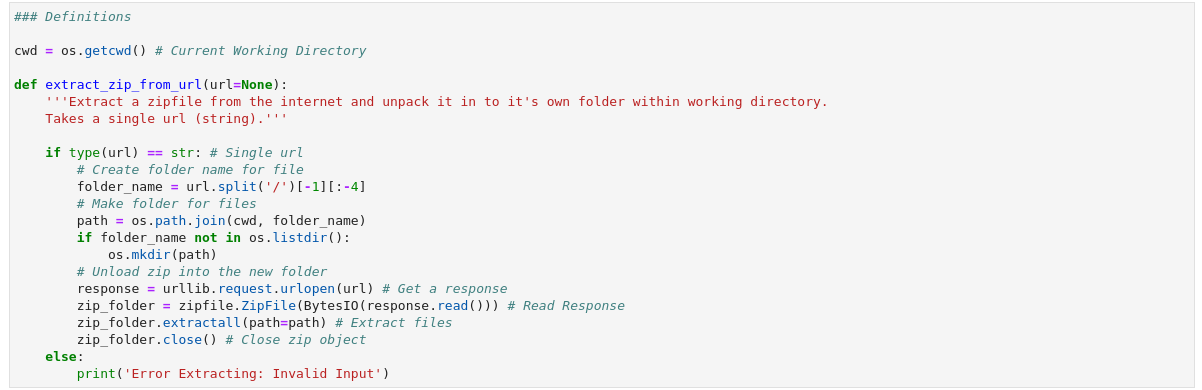
\includegraphics[width=\linewidth]{extractzip}
					\end{minipage}
					\captionof{figure}{A function that extracts and unpacks a zipfile from a url.}
				\end{center}
			\end{minipage}
		}\\
		
	\end{center}
\end{adjustwidth}
\vspace{.5in}

\subsubsection{Minnesota Pollution Control Agency API}

The dataset, Emissions\_MN, was acquired from the MPCA's API. It is a file stored away at this url, \url{'https://files.pca.state.mn.us/pub/file_requests/datasets/Air/PointSourceAirEmissionsInventory.zip'}. This zipfile can be retrieved and unpacked using the function in figure 5.  Within this zipfile is an Excel Spreadsheet (.xlsx) which can be read into a Pandas DataFrame with the function, \texttt{pandas.read\_excel()} and the open source package, \texttt{openpyxl}. 

\subsubsection{PurpleAir API}

This API was very similar to the Google Places API. An API key must be requested and various fields and variables can be utilized to query for real-time data. However, historical data requires special permissions to request by API. The past year of observations within the study area were instead installed manually using the PurpleAir map and download tool. These 524 individual CSV files with very descriptive names of nearby sensors could each be read into a Pandas DataFrame using, \texttt{pandas.read\_csv()}.

\subsection{Data Processing}
\begin{adjustwidth}{-.88in}{-.88in}
	\begin{center}
		\fbox{ % Workflow
			\begin{minipage}{.8\linewidth}
				\begin{center}
					\begin{minipage}{\linewidth}
						\includegraphics[width=\linewidth]{ProcessData}
					\end{minipage}
					\captionof{figure}{Workflow for processing raw data (excluding PurpleAir)}
				\end{center}
			\end{minipage}
		}\\
		
	\end{center}
\end{adjustwidth}
\vspace{.5in}

The code that performs these functions can be found in the folder, \texttt{1\_Data\_IO}, at the end of each dataset's respective notebook.

\subsubsection{Minneapolis Boundary and Study Extent}

Once the CTUs were read into a GeoDataFrame, they could be queried by the field, \texttt{'CTU\_NAME'}. Minneapolis was selected and buffered 26 kilometers. These shapes were saved as \newline \texttt{mpls\_boundary.geojson} and \texttt{study\_extent.geojson}, respectively. 

\subsubsection{Surrounding AADT Segments}

Once AADT\_MN was read into a GeoDataFrame, it was clipped using the function, \newline \texttt{geopandas.clip(gdf, mask)}, where gdf is AADT\_MN and mask is the study extent read as a GeoDataFrame. These polylines were saved as \texttt{aadt.geojson} with all attributes.

\subsubsection{HOLC Grades by Parcel}

HOLC Grades by Parcel were in the correct CRS and within the extent.

\subsubsection{Surrounding MPCA Permitted Emissions}

After the MPCA Permitted Emissions were loaded into a DataFrame, the data was explored extensively, noting the unique years (2006-2020), unique pollutants, and the various ways Portable Source was entered in the \texttt{COUNTY} column. The data was then queried by county. In exploring the latitude and longitude fields, they were found to be flipped. This was corrected and the MPCA notified. Some facilities had NaN coordinate values which sent me on a minor bout of investigative Google API requests. Ultimately, missed locational entries were omitted from the data but there are some leads, (see figure 7).

At this point the queried and corrected permitted emissions DataFrame was spatialized into a Geopandas GeoDataFram using the function, \texttt{geopandas.points\_from\_xy()}, which creates a Geopandas geometry series. The coordinates were reprojected from WGS84 to UTM 15N, NAD83 and then clipped to the extent of the study. These annual emissions were then saved as a CSV, \texttt{emissions.csv}, with new columns 'EASTING' and 'NORTHING' that had values of their reprojected coordinates. \nopagebreak
	\begin{center}
		\fbox{ % Workflow
			\begin{minipage}{.3\linewidth}
				\begin{center}
					\begin{minipage}{\linewidth}
						\includegraphics[width=\linewidth]{suspects}
					\end{minipage}
					\captionof{figure}{\scriptsize{Suspected locations of missed locational entries found through the Google Places API.}}
				\end{center}
			\end{minipage}
		}\\
		
	\end{center}

\subsubsection{PurpleAir}

\begin{adjustwidth}{-.88in}{-.88in}
	\begin{center}
		\fbox{ % Workflow
			\begin{minipage}{.8\linewidth}
				\begin{center}
					\begin{minipage}{\linewidth}
						\includegraphics[width=\linewidth]{ProcessPurpleAir}
					\end{minipage}
					\captionof{figure}{Workflow for processing raw PurpleAir data.}
				\end{center}
			\end{minipage}
		}\\
		
	\end{center}
\end{adjustwidth}
\vspace{.5in}

The 524 individual CSVs from PurpleAir had very descriptive names from which 7 columns were ascertained. This included: latitude, longitude, whether the sensor was outside or not, and if it was a 'B' sensor. The CSVs of the outdoor 'A' sensors were iteratively read into Pandas DataFrames and checked to see if they had a half a year of data. If they did, their indices were recorded for later selection. At this time, start dates, end dates, and number of observations were all recorded for each CSV with the information gathered from the filenames into a DataFrame that looked like figure 8.

\begin{adjustwidth}{-.88in}{-.88in}
	\begin{center}
		\fbox{ % Workflow
			\begin{minipage}{.8\linewidth}
				\begin{center}
					\begin{minipage}{\linewidth}
						\includegraphics[width=\linewidth]{PurpleAirCsvFields}
					\end{minipage}
					\captionof{figure}{Information on the Csv files downloaded from PurpleAir.}
				\end{center}
			\end{minipage}
		}\\
		
	\end{center}
\end{adjustwidth}
\vspace{.5in}

This DataFrame could be selected by the indices of the CSV files that had enough observations. These were considered to be candidates for interpolation. There were 71 using the data downloaded on 10/25/22. These were iterated through to find the average observed PM2.5 levels at each station between the maximum of all Start\_Date (7/24/22) and 10/25/22. There were some outlier sensor readings and these were each removed until 61 sensors were deemed worthy for interpolation. These were spatialized, reprojected, and saved as a CSV, \texttt{pm25\_avg.csv}.

\subsection{Create Template Raster}
\begin{adjustwidth}{-.88in}{-.88in}
	\begin{center}
		\fbox{ % Workflow
			\begin{minipage}{.8\linewidth}
				\begin{center}
					\begin{minipage}{\linewidth}
						\includegraphics[width=\linewidth]{CreateRasterTemplate}
					\end{minipage}
					\captionof{figure}{Workflow to create a template raster.}
				\end{center}
			\end{minipage}
		}\\
		
	\end{center}
\end{adjustwidth}
\vspace{.5in}

In the folder \texttt{2\_Model\_Pollutant\_Exposure} there is a notebook named, \texttt{1\_Raster\_Template} that describes how to perform these steps in more detail. The raster resolution chosen was 50m with 533 x\_cells and 678 y\_cells.

\subsection{Rasterize Emissions Sources}
\begin{adjustwidth}{-.88in}{-.88in}
	\begin{center}
		\fbox{ % Workflow
			\begin{minipage}{.8\linewidth}
				\begin{center}
					\begin{minipage}{\linewidth}
						\includegraphics[width=\linewidth]{RasterizeSources}
					\end{minipage}
					\captionof{figure}{Workflow for rasterizing emissions source data.}
				\end{center}
			\end{minipage}
		}\\
		
	\end{center}
\end{adjustwidth}
\vspace{.5in}

The notebook that rasterizes the pollution sources can be found at \newline \texttt{2\_Model\_Pollutant\_Exposure/2\_Rasterize\_Sources.ipynb}. Notably during this process, the Rasterio function \texttt{features.rasterize()} was found to only have two types of merge algebra options, \texttt{rasterio.enums.MergeAlg.add} and the default, \newline \texttt{rasterio.enums.MergeAlg.replace}. The merge algebra was set to \texttt{.replace} for AADT and \texttt{.add} for the current and cumulative pollutant emissions from this list of pollutants: 'Sulfur Dioxide', 'PM Primary', 'PM10 Primary', 'PM2.5 Primary', 'Volatile Organic Compounds'. These rasters were exported as GeoTiffs into the Rasterized\_Sources folder. 

\subsection{Emissions Dispersion}
\begin{adjustwidth}{-.88in}{-.88in}
	\begin{center}
		\fbox{ % Workflow
			\begin{minipage}{.8\linewidth}
				\begin{center}
					\begin{minipage}{\linewidth}
						\includegraphics[width=\linewidth]{EmissionsDispersion}
					\end{minipage}
					\captionof{figure}{Workflow for dispersing rasterized emissions data.}
				\end{center}
			\end{minipage}
		}\\
		
	\end{center}
\end{adjustwidth}
\vspace{.5in}


Example code that performs these calculations can be found in the notebooks within the folder, \texttt{2\_Model\_Pollutant\_Exposure/3\_Model\_Exposure}. Generally, this involved constructing a non-standardized, Gaussian kernel using the function shown in figure 13 with a fixed diameter, $l$, of 200 cells (10km at 50m resolution) and a sigma (10) to start. This kernel was passed along with a rasterized pollution source raster read as a numpy array into the Scipy function, \texttt{scipy.ndimage.convolve()}. This effectively emulated a weighted focal sum across the pollution source raster where the sigma represents a sort of density or fullness of the kernel (weights) used for dispersion. 


\begin{adjustwidth}{-.88in}{-.88in}
	\begin{center}
		\fbox{ % Workflow
			\begin{minipage}{.8\linewidth}
				\begin{center}
					\begin{minipage}{\linewidth}
						\includegraphics[width=\linewidth]{kernelfct}
					\end{minipage}
					\captionof{figure}{A function that creates a non-standardized, Gaussian Kernel with specified diameter and sigma.}
				\end{center}
			\end{minipage}
		}\\
		
	\end{center}
\end{adjustwidth}
\vspace{.5in}

After the dispersion took place, the resulting values were divided by their maximum value to normalize the data. This was considered to be the exposure raster for each respective source and all were saved in the folder, \texttt{2\_Model\_Pollutant\_Exposure/\_Modeled\_Exposure}. The distribution of the raster values for \texttt{aadt\_exposure.tif} and \newline \texttt{PM2.5 Primary\_current\_exposure.tif} can be seen in figure 14. 

\vspace{.5in}
\begin{adjustwidth}{-.88in}{-.88in}
\begin{center}
	\fbox{ % Workflow
		\begin{minipage}{.95\linewidth}
			\begin{multicols}{2}
				\begin{minipage}{\linewidth}
					\includegraphics[width=\linewidth]{aadt_norm}
					\scriptsize{\texttt{aadt\_exposure.tif}}
				\end{minipage}
				\begin{minipage}{\linewidth}
					\includegraphics[width=\linewidth]{pm25_norm}
					\scriptsize{\texttt{PM2.5 Primary\_current\_exposure.tif}}
				\end{minipage}
			\end{multicols}
			\captionof{figure}{Distributions of pollution source exposure raster values.}
			
		\end{minipage}
	}\\
	
\end{center}
\end{adjustwidth}

\subsection{Create Hazard Index}
\begin{adjustwidth}{-.88in}{-.88in}
	\begin{center}
		\fbox{ % Workflow
			\begin{minipage}{.8\linewidth}
				\begin{center}
					\begin{minipage}{\linewidth}
						\includegraphics[width=\linewidth]{CreateHazardIndex}
					\end{minipage}
					\captionof{figure}{Workflow for constructing Current PM2.5 Hazard Indices.}
				\end{center}
			\end{minipage}
		}\\
		
	\end{center}
\end{adjustwidth}
\vspace{.5in}

The code for this portion of the project can be found in the notebooks within, \texttt{3\_Hazard\_Index}. At this stage, it was decided to only use the layers \texttt{aadt\_exposure.tif}, $T$, and \texttt{PM2.5 Primary\_current\_exposure.tif}, $I$, to construct current PM2.5 hazard indices. Linear combinations of these layers were computed using numpy and layer weights between 0\% and 100\% such that $T_{weight} + I_{weight} = \%100$. These test hazard indices were saved in the folder, \texttt{3\_Hazard\_Index/\_Tests}, with the naming format of, \texttt{[$I_{weight}$]PM-[$T_{weight}$]T\_test.tif}. 

\subsection{Validate Hazard Index}
\begin{adjustwidth}{-.88in}{-.88in}
	\begin{center}
		\fbox{ % Workflow
			\begin{minipage}{.8\linewidth}
				\begin{center}
					\begin{minipage}{\linewidth}
						\includegraphics[width=\linewidth]{ValidateHazardIndex}
					\end{minipage}
					\captionof{figure}{Workflow for validating Hazard Indices with PurpleAir Observations.}
				\end{center}
			\end{minipage}
		}\\
		
	\end{center}
\end{adjustwidth}
\vspace{.5in}
Code for this section can be found within the notebooks in the folder, \texttt{4\_Validate\_Index\_Surface}. 

\subsubsection{Interpolation} 

The validation process began with constructing an interpolator for the PurpleAir observed average PM2.5 readings using the Scipy function, \texttt{interpolate.RBFInterpolator()} and the parameters: $y$, $d$, $kernel='thin\_plate\_spline'$, and $smoothing=0.1$ where $y$ is the coordinate pairs from the PurpleAir Stations as a numpy array of shape, (Number of Stations, 2), and $d$ was an array of the 'Avg\_pm2.5' values. This interpolator could be used with the coordinates from \texttt{template.npy} to construct a surface (see figure 17). The resulting values were normalized by their maximum value (see figure 18) and saved as the file, \texttt{PurpleAir\_Interpolation\_Normalized.tif}.

\vspace{.35in}

\begin{adjustwidth}{-.88in}{-.88in}
	\begin{center}
		\fbox{ % Workflow
			\begin{minipage}{.7\linewidth}
				\begin{center}
					\begin{minipage}{\linewidth}
						\includegraphics[width=\linewidth]{interp}
					\end{minipage}
					\captionof{figure}{Code snippet showing the interpolation method used.}
				\end{center}
			\end{minipage}
		}\\
		
	\end{center}
\end{adjustwidth}

\begin{adjustwidth}{-.88in}{-.88in}
	\begin{center}
		\fbox{ % Workflow
			\begin{minipage}{.7\linewidth}
				\begin{center}
					\begin{minipage}{\linewidth}
						\includegraphics[width=\linewidth]{PurpleAirInterpValues}
					\end{minipage}
					\captionof{figure}{Value distribution of \texttt{PurpleAir\_Interpolation\_Normalized.tif}.}
				\end{center}
			\end{minipage}
		}\\
		
	\end{center}
\end{adjustwidth}

\subsubsection{Accuracy Checks}

The interpolation (observed) and hazard indices (predicted) were masked by the total bounds of Minneapolis using the function, \texttt{numpy.ma.array()}. Example code can be seen in figure 19. The residuals between these two masked arrays were computed to find the RMSE of each index within Minneapolis and the residuals spatial and value distributions were visualized. These initial comparisons can be explored further in the notebook, \newline \texttt{4\_Validate\_Index\_Surface/2\_Compare\_Model\_and\_PurpleAir.ipynb}. 
\vspace{.5in}
\begin{adjustwidth}{-.88in}{-.88in}
	\begin{center}
		\fbox{ % Workflow
			\begin{minipage}{.8\linewidth}
				\begin{center}
					\begin{minipage}{\linewidth}
						\includegraphics[width=\linewidth]{maskingpurpleair}
					\end{minipage}
					\captionof{figure}{Masking the PurpleAir interpolation by the total bounds of Minneapolis.}
				\end{center}
			\end{minipage}
		}\\
		
	\end{center}
\end{adjustwidth}
\vspace{.5in}

\subsection{Sensitivity Analysis}
\begin{adjustwidth}{-.88in}{-.88in}
	\begin{center}
		\fbox{ % Workflow
			\begin{minipage}{.8\linewidth}
				\begin{center}
					\begin{minipage}{\linewidth}
						\includegraphics[width=\linewidth]{SensitivityAnalysis}
					\end{minipage}
					\captionof{figure}{Workflow for sensitivity analysis.}
				\end{center}
			\end{minipage}
		}\\
		
	\end{center}
\end{adjustwidth}
\vspace{.5in}

The script that performs this analysis is in the main Final\_Project Directory called, \texttt{7\_Sensitivity Analysis\_Prep.py}. On top of varying the weights for the exposure layers, the Sigma ($\sigma$) in the traffic dispersion Gaussian Kernel was allowed to vary between 1 and 15 by 0.5 intervals with a constant 10km diameter. The naming convention for these hazard indices was changed to: \newline\newline \texttt{[$\sigma$]sig\_[$I_{weight}$]I-[$T_{weight}$]T\_HazardIndex.tif}. \newline\newline Code that explores these findings can be found in the folder \texttt{7\_Sensitivity\_Analysis}.

\subsection{Zonal Statistics}

\begin{adjustwidth}{-.88in}{-.88in}
	\begin{center}
		\fbox{ % Workflow
			\begin{minipage}{.8\linewidth}
				\begin{center}
					\begin{minipage}{\linewidth}
						\includegraphics[width=\linewidth]{ZonalStats}
					\end{minipage}
					\captionof{figure}{Workflow for performing Zonal Statisics with hazard indices.}
				\end{center}
			\end{minipage}
		}\\
		
	\end{center}
\end{adjustwidth}
\vspace{.5in}

The Zonal Means of some select hazard indices were calculated using the HOLC Parcels as zones and the resulting GeoJSONs can be found in the folder, \newline \texttt{7\_Sensitivity\_Analysis/Zonal\_Stats}. Example code that accomplishes this step can be found in \texttt{5\_Zonal\_Statistics/1\_HOLC\_Zones.ipynb} and was included in the senstivity analysis script. Notably, it was discovered that the Rasterstats function, \texttt{zonal\_stats()} does not accept affine transformations with an inverted y-axis. This can be corrected with a function shown in figure 22.

\begin{adjustwidth}{-.88in}{-.88in}
	\begin{center}
		\fbox{ % Workflow
			\begin{minipage}{.7\linewidth}
				\begin{center}
					\begin{minipage}{\linewidth}
						\includegraphics[width=\linewidth]{fliprast}
					\end{minipage}
					\captionof{figure}{A function which flips a raster and affine transformation such that North is "up."}
				\end{center}
			\end{minipage}
		}\\
		
	\end{center}
\end{adjustwidth}
\vspace{.5in}

%To be determined... But for modeling air quality I'm considering using resources from both \href{https://www.pca.state.mn.us/business-with-us/air-quality-modeling}{MPCA}  and \href{https://plumepgh.org/model_data.html}{Plume Pittsburg}. I think the model validation will involve some RMSE, residual, and Pearson Correlation calculations. For the correlation analysis, I was thinking of doing something similar to an earlier project of mine using SLX, SLY, Durbin, and different GWR spatial regressions, but I'm open to suggestions! MPCA also has an \href{https://www.pca.state.mn.us/business-with-us/air-emissions-risk-analysis-aera}{air emissions risk assessment} that I will explore further when considering the risk index.

\section{Results}

\begin{adjustwidth}{-.88in}{-.88in}
	\begin{center}
		\fbox{ % Workflow
			\begin{minipage}{.95\linewidth}
				\begin{center}
					\begin{minipage}{\linewidth}
						\includegraphics[width=\linewidth]{Purple Air Interpolation}
					\end{minipage}
					\captionof{figure}{Interpolation of Average PM2.5 Observations with sample points displayed ($\frac{\mu g}{m^3}$).}
				\end{center}
			\end{minipage}
		}\\
		
	\end{center}
\end{adjustwidth}

\begin{adjustwidth}{-.88in}{-.88in}
	\begin{center}
		\fbox{ % Workflow
			\begin{minipage}{.95\linewidth}
				\begin{center}
					\begin{minipage}{\linewidth}
						\includegraphics[width=\linewidth]{15.0sig_40I-60T_HazardIndex}
					\end{minipage}
					\captionof{figure}{Hazard index with traffic dispersion sigma of 15 (40\% Current PM2.5 Industrial Emissions, 60\% Current Traffic).}
				\end{center}
			\end{minipage}
		}\\
		
	\end{center}
\end{adjustwidth}

\begin{adjustwidth}{-.88in}{-.88in}
	\begin{center}
		\fbox{ % Workflow
			\begin{minipage}{.95\linewidth}
				\begin{center}
					\begin{minipage}{.95\linewidth}
						\includegraphics[width=\linewidth]{Sensitivity}
					\end{minipage}
					\captionof{figure}{Graphs showing relationships between RMSE of hazard indices over normalized interpolated values, sigma of traffic dispersion, and weight of the traffic exposure layer.}
				\end{center}
			\end{minipage}
		}\\
		
	\end{center}
\end{adjustwidth}
\begin{adjustwidth}{-.88in}{-.88in}
	\begin{center}
		\fbox{ % Workflow
			\begin{minipage}{.95\linewidth}
				\begin{multicols}{2}
					\begin{minipage}{\linewidth}
						\includegraphics[width=\linewidth]{15.0sig_40I-60T_HazardIndex}
						\scriptsize{40\% Current PM2.5 Industrial Emissions, 60\% Current Traffic}
					\end{minipage}
					\begin{minipage}{\linewidth}
						\includegraphics[width=\linewidth]{15.0sig_60I-40T_HazardIndex}
						\scriptsize{60\% Current PM2.5 Industrial Emissions, 40\% Current Traffic}
					\end{minipage}
				\end{multicols}
					\captionof{figure}{Comparison of hazard indices with traffic dispersion sigma of 15.}

			\end{minipage}
		}\\
		
	\end{center}
\end{adjustwidth}

\begin{adjustwidth}{-.88in}{-.88in}
	\begin{center}
		\fbox{ % Workflow
			\begin{minipage}{.9\linewidth}
				\begin{multicols}{2}
					\begin{minipage}{\linewidth}
						\includegraphics[width=\linewidth]{15.0sig_40I-60T_HazardIndex Residuals}
						\scriptsize{40\% Current PM2.5 Industrial Emissions, 60\% Current Traffic}
					\end{minipage}
					\begin{minipage}{\linewidth}
						\includegraphics[width=\linewidth]{15.0sig_60I-40T_HazardIndex Residuals}
						\scriptsize{60\% Current PM2.5 Industrial Emissions, 40\% Current Traffic}
					\end{minipage}
				\end{multicols}
				\captionof{figure}{Comparison of hazard indices' residuals (traffic dispersion sigma of 15) from normalized average \newline PurpleAir observations.}
				
			\end{minipage}
		}\\
		
	\end{center}
\end{adjustwidth}

\begin{adjustwidth}{-.88in}{-.88in}
	\begin{center}
		\fbox{ % Workflow
			\begin{minipage}{.9\linewidth}
				\begin{multicols}{2}
					\begin{minipage}{\linewidth}
						\includegraphics[width=\linewidth]{15.0sig_40I-60T_HazardIndex Zonal Statistics}
						\scriptsize{40\% Current PM2.5 Industrial Emissions, 60\% Current Traffic}
					\end{minipage}
					\begin{minipage}{\linewidth}
						\includegraphics[width=\linewidth]{15.0sig_60I-40T_HazardIndex Zonal Statistics}
						\scriptsize{60\% Current PM2.5 Industrial Emissions, 40\% Current Traffic}
					\end{minipage}
				\end{multicols}
				\captionof{figure}{Comparison of hazard indices zonal means (traffic dispersion sigma of 15) with HOLC parcels.}
				
			\end{minipage}
		}\\
		
	\end{center}
\end{adjustwidth}

\begin{adjustwidth}{-.88in}{-.88in}
	\begin{center}
		\fbox{ % Workflow
			\begin{minipage}{.95\linewidth}
					\begin{minipage}{\linewidth}
						\includegraphics[width=\linewidth]{15.0sig_40I-60T_HazardIndex Index Mean}
					\end{minipage}
				\captionof{figure}{Hazard index zonal mean average value by HOLC Grade (traffic dispersion sigma of 15, \newline 40\% Current PM2.5 Industrial Emissions, 60\% Current Traffic).}
				
			\end{minipage}
		}\\
		
	\end{center}
\end{adjustwidth}

\begin{adjustwidth}{-.88in}{-.88in}
	\begin{center}
		\fbox{ % Workflow
			\begin{minipage}{.95\linewidth}
				\begin{minipage}{\linewidth}
					\includegraphics[width=\linewidth]{15.0sig_60I-40T_HazardIndex Index Mean}
				\end{minipage}
				\captionof{figure}{Hazard index zonal mean average value by HOLC Grade (traffic dispersion sigma of 15, \newline 60\% Current PM2.5 Industrial Emissions, 40\% Current Traffic).}
				
			\end{minipage}
		}\\
		
	\end{center}
\end{adjustwidth}


%\begin{adjustwidth}{-.55in}{-.55in}	
%
%	\fbox{\begin{minipage}{\linewidth} 
%			\begin{minipage}{.5\linewidth}
%				\includegraphics[width=\linewidth]{0PM-100T_index}
%			\end{minipage}
%			\begin{minipage}{.5\linewidth}
%				\includegraphics[width=\linewidth]{100PM-0T_index}
%			\end{minipage}
%			\captionof{figure}{Visualizations of Normalized $T_{2022}$ (Left) and Transformed \& Normalized $I_{2020}$ PM2.5 emissions (Right).}
%	\end{minipage}}
	
%\end{adjustwidth}

%\newpage
%\begin{adjustwidth}{-.55in}{-.55in}	
%	\fbox{ 
%		\begin{minipage}{\linewidth}
%			\begin{center}
%				\begin{minipage}{\linewidth}
%					\includegraphics[width=\linewidth]{50PM-50T_index.png}
%				\end{minipage}
%				\captionof{figure}{An example of an environmental hazard cost surface (50\% Current Traffic, 50\% Current PM2.5 Emissions).}
%			\end{center}
%		\end{minipage}
%		
%	}
%\end{adjustwidth}
%

%\begin{tabular}{lrrrrr}
%	\hline
%	{} &     $R^2$ &  Pearson Coeff &     p-value &  Residual Morans I &     p-value \\
%	\hline
%	NonSpatial &  0.0888 &         0.2980 &  3.7698e-09 &             0.4336 &  1.1466e-18 \\
%	SLX        &  0.1041 &         0.3226 &  1.4926e-10 &             0.4393 &  3.5773e-19 \\
%	SLY        &  0.2682 &         0.5179 &  3.4336e-27 &            -0.0877 &  8.9419e-02 \\
%	Durbin     &  0.2673 &         0.5170 &  4.3190e-27 &            -0.0774 &  1.3412e-01 \\
%	GWR        &  0.4777 &         0.6959 &  9.7322e-56 &            -0.4243 &  7.2401e-18 \\
%	\hline
%\end{tabular}
%\captionof{table}{Accuracy checks of regressions. Regressand: $T$, Regressor: $R_{NW}$.}
%\vspace{.2in}
%\begin{adjustwidth}{-.55in}{}
%	\begin{tabular}{lrrrrllll}
%		\hline
%		{} &  CONSTANT &       p-value &  $R_{NW}$ &      p-value & $R_{NW}$\_lag &  p-value & $T$\_lag & p-value \\
%		\hline
%		NonSpatial &  33.44931 &  1.98079e-135 &      -0.12088 &  3.76979e-09 &                - &        - &              - &       - \\
%		SLX        &  34.99942 &  8.84001e-115 &      -0.05236 &  1.21008e-01 &         -0.11258 &  0.01219 &              - &       - \\
%		SLY        &  12.48954 &   5.28596e-07 &      -0.05557 &  3.39681e-03 &                - &        - &        0.63771 &     0.0 \\
%		Durbin     &  13.00777 &   4.13289e-06 &      -0.04503 &  1.39290e-01 &         -0.01866 &  0.65725 &        0.62976 &     0.0 \\
%		\hline
%	\end{tabular}
%	\captionof{table}{Coefficients of regression models. Regressand: $T$, Regressor: $R_{NW}$.}
%	
%\end{adjustwidth}


\section{Discussion and Future Directions}
	
	This project utilized a wide range of geographic information science techniques. Due to this, there are a number of steps in the workflow that could be improved.
	
	In reviewing the PurpleAir interpolation visually (figure 23), we can see that the spline technique made semi-reasonable predictions. However, upon reviewing literature on modeling air pollution at street level, interpolating air quality data at this fine of scale can be quite difficult. \textcite{FOREHEAD} states, "Concentrations can be highly variable over short distances and intervals of time, due to fleet composition, congestion, weather (mainly wind) and the shape of street canyons." Even at this temporal resolution, there can be many confounding factors not included in the interpolator used. This part of the analysis could certainly be improved upon, and future directions of this research will definitely involve further scrutiny of this step.
	
	The hazard index itself was a bit of an experiment. The ultimate goal was to try and include traffic levels in air quality dispersion modeling which are typically only factored into the ambient air quality in MPCA \href{https://www.pca.state.mn.us/sites/default/files/aq2-58.pdf}{Dispersion Modeling}. As can be seen in figure 26, the higher index values were primarily along roadways with much of the study area having an index less than 0.3. Looking at the residual plots (figure 27), we can see that the index was consistently lower than the normalized interpolated values (positive residuals) leading me to wonder about including more sources (such as rail yards) and perhaps including an ambient hazard index level based on the distribution of the residuals (see figure 27 histograms). 
	
	Other clues to improve the index come from looking at the results of the sensitivity analysis (see figure 25). Here, we can see two definite patterns. One, the greater the sigma value for traffic, the more accurate the model appeared. Two, the indices that weighted traffic appeared to perform better as they generally had higher index values. When I ran the dispersion models on my computer, my memory (16Gb) maxed out when using a sigma of 15 at the constant diameter of 10km. Perhaps utilizing a supercomputer to perform sensitivity analysis with larger sigmas, larger diameters, different sigmas for industrial pollution, and more refined weights could lead to a more accurate hazard index.
	
	The zonal statistics were a good way to tie this analysis back to the problem statement. We did see in figures 29 and 30 that the different HOLC grades tended to have average indices that aligned with what we could hypothesize from history. However, I think that improving the model should take precedence before giving these values much consideration. Future directions could include ANOVA analysis of the HOLC grades and using different zones (such as Census Block Groups) to conduct correlation analyses.
	
	Further directions for this work should include a spatio-temporal investigation of the index to better understand temporally-cumulative impacts of PM2.5 and whether or not things are improving. Community engagement is also key, as the pollutants to focus on in the future should largely reflect what people care about (co-creation). Educational resources should also be developed further to assist in the big campaign to tackle these disparities in pollution exposure that the City of Minneapolis' offices of Sustainability and Health are starting.
	
	Environmental justice (EJ) continues to expand and incorporate different conceptions of space, environment, and justice. Contemporary EJ writers often cite a need for more community outreach, education, and inclusive decision-making as well as innovative collaboration between planners, policy-makers, academics, and citizens to achieve profound environmental justice \cite{walker2010, corburn2003, pearsall2010}. \textcite{pearsall2010} emphasize a need for well defined indicators that are spatially focused, not aggregate measures, to gauge a policy's success at implementing environmental justice. This new workflow and index are a couple more tools we can use to collectively reckon with our history, assess our current situation, and work toward reparations. 
	
\newpage
\begingroup           % Ctrl T to uncomment
\setstretch{1}
\setlength\bibitemsep{12pt}  % length between two different entries
\printbibliography
\endgroup

\section*{Self Score}
\setstretch{.2}
\begin{tabular}{|p{.2\linewidth}|p{.2\linewidth}|p{.2\linewidth}|p{.1\linewidth}|}
	\hline
	\textbf{Category}            & \textbf{Description}                                                                                                                                                                                                                                                                                                                                              & \textbf{Points Possible} & \textbf{Score} \\ \hline
\vspace{.2in}\textbf{Structural Elements} & {\tiny All elements of a lab report are included (2 points each): Title, Notice: Dr. Bryan Runck, Author, Project Repository, Date, Abstract, Problem Statement, Input Data w/ tables, Methods w/ Data, Flow Diagrams, Results, Results Verification, Discussion and Conclusion, References in common format, Self-score}                                        & \vspace{.2in}28              &   \vspace{.2in}26    \\ \hline
	\vspace{.2in}\textbf{Clarity of Content}  & {\tiny Each element above is executed at a professional level so that someone can understand the goal, data, methods, results, and their validity and implications in a 5 minute reading at a cursory-level, and in a 30 minute meeting at a deep level (12 points). There is a clear connection from data to results to discussion and conclusion (12 points).} & \vspace{.2in}24              &  \vspace{.2in}20     \\ \hline
	\vspace{.2in}\textbf{Reproducibility}     & {\tiny Results are completely reproducible by someone with basic GIS training. There is no ambiguity in data flow or rationale for data operations. Every step is documented and justified.}                                                                                                                                                                     & \vspace{.2in}28              &     \vspace{.2in}20  \\ \hline
	\vspace{.2in}\textbf{Verification}        & {\tiny Results are correct in that they have been verified in comparison to some standard. The standard is clearly stated (10 points), the method of comparison is clearly stated (5 points), and the result of verification is clearly stated (5 points).}                                                                                                      & \vspace{.2in}20              &   \vspace{.2in}17    \\ \hline
	&                                                                                                                                                                                                                                                                                                                                                          & \vspace{.02in}100             &   \vspace{.02in}83     \\ \hline
\end{tabular}
\end{document}